\chapter{Antecedentes}\label{chapter02}

La investigación sobre predicción de demanda para productos perecederos ha avanzado con rapidez en los últimos años gracias a la IA. En el ámbito del comercio de alimentos frescos en línea, se ha demostrado que la incorporación de variables como el clima y el calendario mejora significativamente la precisión de los modelos predictivos (Ni et al., 2022). Posteriormente, investigaciones más recientes en el sector minorista alimentario evidencian que modelos basados en redes neuronales recurrentes, como LSTM, superan sistemáticamente a los enfoques estadísticos tradicionales al minimizar tanto los faltantes como los excesos de inventario (Nassibi et al., 2023). Estos avances reflejan el papel creciente de la inteligencia artificial en la optimización de la gestión de productos perecederos. Aun así, en Argentina se sigue desaprovechando el 12,5\% de la producción agroalimentaria, de las que solo el 1,2\% se pierden en la etapa comercial. El impacto se vuelve crítico en rubros como panaderías y pastelerías, donde en 2024 cerraron más de 400 locales y las ventas de pan cayeron un 53\%.


\section{Marco teórico}

En esta sección se describen los fundamentos conceptuales y técnicos necesarios para comprender el enfoque del sistema propuesto, incluyendo tecnologías de predicción, Inteligencia artificial, aprendizaje automático y su aplicación en la predicción de demanda, y problemáticas sociales vinculadas al desperdicio de alimentos, que son relevantes para el sistema a desarrollar.


\subsection{Inteligencia artificial}

La inteligencia artificial (en adelante IA) es un campo de estudio dentro de la informática que busca desarrollar sistemas capaces de realizar tareas que normalmente requieren inteligencia humana, tales como el razonamiento, la percepción, la toma de decisiones o el aprendizaje. El término fue acuñado formalmente en 1956 durante la conferencia de Dartmouth, considerada el punto de partida de la disciplina \parencite{mccarthy1955}.\\

En términos generales, la IA puede dividirse en dos grandes enfoques:

\begin{itemize}
    \item \textbf{IA débil} (\textit{narrow AI}): especializada en tareas concretas como traducción automática, recomendación de productos o reconocimiento de imágenes \parencite{russell2021}.
    
    \item \textbf{IA fuerte} (\textit{general AI}): de carácter hipotético, orientada a replicar el razonamiento humano en su totalidad \parencite{russell2021}.
\end{itemize}

Gracias al aumento en la capacidad de cómputo y al acceso a grandes volúmenes de datos, el desarrollo reciente de IA basada en aprendizaje automático (\textit{machine learning}) ha permitido avances significativos en múltiples industrias, incluyendo salud, finanzas, logística y comercio minorista \parencite{jordan2015}.

Estos avances han dado lugar al uso extendido de IA en tareas de predicción de demanda, optimización de recursos y automatización de procesos, tal como se propone en el presente proyecto.

La IA también se ha convertido en una herramienta clave para abordar problemáticas socioambientales, como el desperdicio de alimentos, al permitir el análisis en tiempo real de patrones de consumo y la generación de alertas y recomendaciones \parencite{rolnick2019}.

\subsection{Aprendizaje automático}

El aprendizaje automático (\textit{machine learning}, en adelante ML) es una subárea de la inteligencia artificial que se enfoca en desarrollar algoritmos capaces de aprender automáticamente a partir de datos, identificar patrones y realizar predicciones o tomar decisiones sin ser programados explícitamente para cada tarea específica \parencite{mitchell1997}.

En contraste con la programación tradicional —donde se define explícitamente cada regla—, en ML los sistemas ajustan su comportamiento a partir de ejemplos y experiencia previa, lo que permite adaptarse a entornos dinámicos o impredecibles. Existen tres grandes categorías de aprendizaje automático:

\begin{itemize}
    \item \textbf{Supervisado}: el modelo se entrena con datos etiquetados, es decir, conjuntos de datos en los que cada entrada está asociada a una salida conocida. (por ejemplo, ventas históricas con cantidades reales).
    
    \item \textbf{No supervisado}: busca patrones o agrupamientos en datos no etiquetados.
    
    \item \textbf{Por refuerzo}:  el agente aprende a tomar decisiones mediante un sistema de recompensas y penalizaciones asociadas a sus acciones dentro de un entorno. \parencite{sutton2018}.
\end{itemize}

En el ámbito de la predicción de demanda y la gestión comercial, el ML ha demostrado ser altamente efectivo. Algoritmos como regresiones, árboles de decisión, \textit{random forest}, redes neuronales o XGBoost permiten prever comportamientos complejos en entornos de alta variabilidad, como el retail alimentario o los productos perecederos \parencite{carbonneau2008}.

Gracias a su capacidad para adaptarse a datos históricos y variables externas —como el clima, promociones o eventos locales—, el ML se ha convertido en una herramienta estratégica para reducir mermas, optimizar la producción y tomar decisiones basadas en evidencia, alineándose con los objetivos del presente proyecto.

\subsection{Series temporales}

Una serie temporal es una secuencia de observaciones recolectadas en intervalos regulares a lo largo del tiempo. Este tipo de datos permite analizar la evolución de un fenómeno y modelar su comportamiento futuro mediante técnicas estadísticas o de aprendizaje automático \parencite{chatfield2004}. En el caso del comercio minorista, las ventas históricas diarias o semanales de un producto conforman una serie temporal típica.\\

Las series temporales suelen contener tres componentes principales:

\begin{itemize}
    \item \textbf{Tendencia (\textit{trend})}: dirección general del movimiento a largo plazo.
    
    \item \textbf{Estacionalidad (\textit{seasonality})}: patrones repetitivos dentro de un periodo (como días de la semana o estaciones).
    
    \item \textbf{Ruido (\textit{noise})}: variaciones aleatorias e impredecibles.
\end{itemize}

La predicción de series temporales es crucial para aplicaciones como la planificación de la producción, gestión de inventarios y optimización de recursos, ya que permite anticiparse a picos o caídas en la demanda \parencite{hyndman2018}.

Tradicionalmente, se utilizaron modelos como ARIMA, Holt-Winters y modelos exponenciales suavizados, aunque en la actualidad han ganado terreno los modelos basados en aprendizaje automático y redes neuronales, especialmente cuando se incorporan variables exógenas como el clima o eventos especiales \parencite{bandara2020}.

En el presente proyecto, las series temporales constituyen la estructura central sobre la cual se apoyará la generación de predicciones de demanda, mediante el uso de modelos ya existentes y herramientas que permiten adaptarse dinámicamente a los patrones observados en los datos históricos y en el contexto operativo del comercio.

\subsection{Modelos de predicción}

Los modelos de predicción son herramientas matemáticas o computacionales que permiten estimar el valor futuro de una variable en función de sus observaciones pasadas y/o de otras variables relacionadas. En el contexto de series temporales, estos modelos se utilizan para anticipar comportamientos futuros de fenómenos que evolucionan en el tiempo, como la demanda de productos perecederos en comercios minoristas \parencite{hyndman2018}.

Entre los enfoques tradicionales más utilizados se encuentran:

\begin{itemize}

    \item \textbf{Regresión}: es una técnica utilizada en estadística y aprendizaje automático que permite modelar y predecir el valor de una variable dependiente en función de una o más variables independientes. Su objetivo principal es identificar y cuantificar la relación existente entre dichas variables.

    \item \textbf{Regresión lineal}: es la forma más básica de regresión, que asume una relación lineal entre las variables. Modela esta relación mediante una recta que minimiza la diferencia entre los valores observados y los valores predichos. Es especialmente útil en contextos donde los datos presentan una estructura simple y relaciones directas. Sin embargo, su capacidad para capturar patrones complejos o no lineales es limitada, lo que restringe su aplicación en problemas con dinámicas más sofisticadas.
    
    \item \textbf{ARIMA (AutoRegressive Integrated Moving Average)}: combina componentes autorregresivos, de promediado móvil y diferenciación para tratar series no estacionarias \parencite{box2015}.
    
    \item \textbf{Holt-Winters}: extensión del suavizado exponencial que incorpora estacionalidad y tendencia, útil para pronósticos a corto plazo con ciclos estables.
\end{itemize}

Estos modelos son apreciados por su simplicidad y bajo costo computacional, aunque presentan limitaciones cuando hay muchas variables externas o relaciones no lineales.

Con el auge del aprendizaje automático, se han incorporado técnicas más complejas que permiten capturar relaciones no lineales y variables exógenas:

\begin{itemize}
    \item \textbf{Prophet}: modelo desarrollado por Facebook que permite ajustar estacionalidades múltiples y eventos especiales de forma flexible \parencite{taylor2018}.
    
    \item \textbf{LSTM (Long Short-Term Memory)}: tipo de red neuronal recurrente capaz de aprender dependencias de largo plazo, muy utilizada en predicción de series temporales con datos ruidosos o variables múltiples (Hewamalage, 2021).
\end{itemize}

Como se observa en la Figura~\ref{fig:lstm}, esta arquitectura permite mantener y transmitir información a lo largo del tiempo, lo cual la hace especialmente útil para modelar secuencias con relaciones temporales complejas.

\begin{figure}[t]
    \centering
    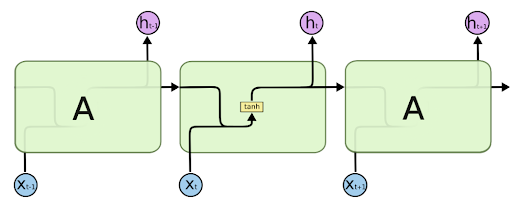
\includegraphics[width=0.7\textwidth]{images/lstm.png}
    \caption{LSTM (Long Short-Term Memory) básico.}
    \label{fig:lstm}
\end{figure}

\begin{itemize}
    \item \textbf{Transformers}: arquitectura inicialmente desarrollada para procesamiento de lenguaje natural, que ha comenzado a aplicarse con éxito en predicción multivariada de series temporales \parencite{li2019}.
\end{itemize}

La elección del modelo dependerá del tipo de datos disponibles, la granularidad deseada y los requisitos de interpretabilidad y precisión. En este proyecto, estos modelos permitirán estimar con mayor exactitud la demanda diaria de productos, reduciendo mermas y ajustando la producción a las condiciones reales del entorno.

\subsection{Evaluación de modelos predictivos}

La evaluación de modelos predictivos es un paso fundamental en el desarrollo de soluciones basadas en inteligencia artificial o series temporales, ya que permite medir cuán precisas y útiles son las predicciones generadas. Para problemas de regresión —como la predicción de demanda— se utilizan principalmente métricas de error que comparan los valores predichos con los observados.

Entre las más utilizadas se encuentran:

\begin{itemize}
    \item \textbf{MAE (Mean Absolute Error)}: mide el promedio de los errores absolutos entre las predicciones $\hat{y}_t$ y los valores reales $y_t$ \parencite{willmott2005}.
    
    \begin{align}
        \text{MAE} = \frac{1}{n} \sum_{t=1}^{n} \left| y_t - \hat{y}_t \right|
    \end{align}

    \item \textbf{RMSE (Root Mean Squared Error)}: calcula la raíz cuadrada del promedio de los errores al cuadrado, penalizando más fuertemente los errores grandes \parencite{chai2014}.
    
    \begin{align}
        \text{RMSE} = \sqrt{ \frac{1}{n} \sum_{t=1}^{n} \left( y_t - \hat{y}_t \right)^2 }
    \end{align}

    \item \textbf{MAPE (Mean Absolute Percentage Error)}: expresa el error como un porcentaje del valor real. Es útil para comparar modelos en distintas escalas, aunque puede ser inestable cuando $y_t \approx 0$ \parencite{myttenaere2016}.
    
    \begin{align}
        \text{MAPE} = \frac{100}{n} \sum_{t=1}^{n} \left| \frac{y_t - \hat{y}_t}{y_t} \right|
    \end{align}
\end{itemize}

La elección de la métrica depende del contexto. El MAE es más interpretable para usuarios no técnicos, mientras que el RMSE resulta más sensible a errores significativos. 

Estas herramientas también permiten monitorear el desempeño del modelo en producción, facilitando el mantenimiento de su precisión a lo largo del tiempo.

\subsection{Reconocimiento óptico de caracteres}

\indent El Reconocimiento Óptico de Caracteres (OCR) es una tecnología que permite convertir texto impreso o manuscrito en imágenes digitales en texto editable y procesable por máquinas. Es ampliamente utilizada en tareas como la digitalización de documentos, la lectura automatizada de facturas, tickets, formularios y libros (Smith, 2007).

\indent Inicialmente, los sistemas OCR se basaban en técnicas de procesamiento de imágenes y plantillas estáticas, lo que limitaba su capacidad para adaptarse a diferentes formatos, caligrafías o niveles de ruido. Sin embargo, los avances en aprendizaje profundo han revolucionado esta tecnología: los modelos actuales, como CRNN (Convolutional Recurrent Neural Network) y los basados en transformers como TrOCR, ofrecen una mayor precisión y robustez en entornos no estructurados, como fotos tomadas con teléfonos móviles o documentos parcialmente dañados (Baek et al., 2019; Li et al., 2021).

\indent El OCR es especialmente valioso en contextos donde los usuarios no pueden o no desean realizar carga manual de datos, como en pequeños comercios. Al automatizar la lectura de registros de venta o remitos mediante fotos, se reduce la carga operativa y se mejora la calidad del dato ingresado (Khandelwal et al., 2020).

\indent En este proyecto, el OCR cumple un rol clave al permitir a los comerciantes digitalizar información histórica de ventas sin conocimientos técnicos, usando simplemente una fotografía desde la plataforma web, lo cual democratiza el acceso a herramientas de predicción.


\subsection{Modelos de lenguaje extensos}

\indent Los Modelos de Lenguaje Extensos (Large Language Models, LLM) son un tipo avanzado de modelo de IA entrenado con enormes cantidades de texto para comprender, generar y manipular lenguaje natural de forma coherente y contextual. Se basan en arquitecturas como transformers, que han demostrado ser altamente eficaces para tareas complejas de procesamiento del lenguaje natural (Vaswani et al., 2017).

\indent Los LLM aprenden a predecir la siguiente palabra en una secuencia, lo que les permite ejecutar tareas como generación de texto, traducción, resumen automático, respuestas a preguntas y análisis semántico. Modelos como GPT-3, PaLM, BERT o LLaMA han alcanzado niveles de rendimiento cercanos al humano en una variedad de benchmarks lingüísticos (Brown et al., 2020; OpenAI, 2023).

\indent Una de las aplicaciones emergentes de los LLM es su integración con otros flujos de datos no estructurados, como imágenes o documentos escaneados, lo que los convierte en una herramienta poderosa para la automatización de tareas que antes requerían intervención humana. En combinación con OCR y pipelines de extracción, los LLM pueden interpretar textos ambiguos y corregir errores, almacenando la información en forma de tensores (Touvron et al., 2023).

\indent En el contexto de este proyecto, los LLM permiten automatizar la carga de registros de ventas a partir de imágenes, interpretar consultas del usuario en lenguaje natural a través de un chatbot y ofrecer respuestas explicativas, todo sin requerir conocimientos técnicos del usuario final.

\subsection{Chatbots conversacionales}

Los chatbots conversacionales son sistemas informáticos diseñados para interactuar con los usuarios mediante lenguaje natural, ya sea por texto o voz. Su objetivo principal es simular una conversación humana para asistir, informar, resolver consultas o ejecutar acciones específicas dentro de una plataforma digital \parencite{radziwill2017}.

Originalmente basados en reglas fijas y árboles de decisión, los chatbots han evolucionado significativamente gracias a los avances en procesamiento de lenguaje natural (PLN), generación de lenguaje natural (GLN) y, más recientemente, en modelos de lenguaje extensos (or Large Language Models,LLM). Estas tecnologías les permiten comprender intenciones y entidades, responder con mayor coherencia y adaptarse al contexto de las interacciones \parencite{shum2018}.

Existen distintos tipos de chatbots, entre ellos:

\begin{itemize}
    \item \textbf{Chatbots basados en reglas}: operan sobre flujos de conversación predefinidos.
    
    \item \textbf{Chatbots con IA}: utilizan algoritmos de aprendizaje automático, PLN y GLN para entender y generar respuestas dinámicas.
    
    \item \textbf{Chatbots híbridos}: combinan ambos enfoques, lo que los hace flexibles y eficientes.
\end{itemize}

En aplicaciones empresariales, los chatbots se utilizan cada vez más para consultas sobre datos, gestión de operaciones y soporte a decisiones, especialmente en entornos con usuarios no técnicos. Estudios recientes demuestran que la incorporación de asistentes conversacionales mejora la adopción de sistemas analíticos complejos, reduce barreras de entrada y mejora la experiencia del usuario \parencite{knote2021}.

En este proyecto, el chatbot actuará como interfaz principal del sistema, permitiendo al comerciante consultar predicciones de demanda, indicadores clave (KPIs), alertas de sobreproducción y sugerencias de acción, sin necesidad de navegar por menús complejos ni interpretar gráficos técnicos.

\subsection{Bases de datos relacionales y vectoriales}

Las bases de datos relacionales (RDB, por sus siglas en inglés) son estructuras de almacenamiento que organizan la información en tablas con filas y columnas, siguiendo un modelo basado en el álgebra relacional, propuesta por Edgar F. Codd en 1970. Este modelo formaliza las operaciones sobre conjuntos de datos utilizando el concepto de relación, y se convirtió en el estándar dominante para almacenar información estructurada en sistemas informáticos \parencite{codd1970}. 

Las bases relacionales permiten realizar consultas complejas mediante lenguajes como SQL y son ampliamente utilizadas en aplicaciones empresariales debido a su robustez, integridad referencial y facilidad de acceso \parencite{coronel2020}.

En contraposición, las bases de datos vectoriales son un tipo más reciente de almacenamiento orientado a datos no estructurados o semiestructurados representados como tensores. Su principal aplicación está en sistemas que utilizan inteligencia artificial, especialmente modelos de lenguaje, visión por computadora y recuperación semántica, donde se requiere comparar elementos no por igualdad exacta, sino por similitud de contexto o significado \parencite{johnson2019}.

Estos vectores se obtienen comúnmente a través de \textit{embeddings} generados por modelos como Word2Vec, BERT o CLIP, y se almacenan en motores especializados como FAISS, Milvus o Pinecone, optimizados para búsquedas por proximidad (\textit{nearest neighbor search}).

En el contexto de este proyecto, las bases relacionales serán utilizadas para almacenar información estructurada como productos, ventas, fechas y predicciones, mientras que las bases vectoriales podrían emplearse en versiones futuras para mejorar el rendimiento del chatbot, permitiéndole recuperar respuestas basadas en similitud semántica entre preguntas y registros históricos o documentación del sistema.

\subsection{Desperdicio de alimentos}

El desperdicio de alimentos hace referencia a la pérdida de productos aptos para el consumo humano que son descartados, deteriorados o no utilizados en etapas finales de la cadena alimentaria, como la comercialización, el almacenamiento o el consumo doméstico. Se diferencia de la pérdida de alimentos, que ocurre en fases anteriores como la producción, poscosecha o procesamiento (FAO, 2019).

A nivel mundial, se estima que alrededor del 17\% de los alimentos disponibles para los consumidores se desperdicia, lo que representa no solo un problema ético y de seguridad alimentaria, sino también una amenaza ambiental por el uso innecesario de recursos como agua, tierra y energía, y la generación de gases de efecto invernadero \parencite{unep2021}.

En Argentina, se pierde o desperdicia el 12{,}5\% de la producción agroalimentaria, lo que equivale a aproximadamente 16 millones de toneladas por año, con consecuencias económicas directas para todos los actores de la cadena de valor \parencite{tiscornia2022}. Particularmente en supermercados, autoservicios y comercios de proximidad, estudios recientes estiman que las pérdidas en categorías frescas superan el 3\% de la facturación, debido a sobreproducción, quiebres de stock, manipulación inadecuada o falta de planificación \parencite{weteam2021}.

Estas cifras revelan la importancia de implementar soluciones basadas en inteligencia artificial y analítica de datos para alinear la producción con la demanda real, evitar el sobrante no comercializable y aumentar la eficiencia operativa. Además, el combate al desperdicio de alimentos contribuye directamente al cumplimiento del Objetivo de Desarrollo Sostenible (ODS) 12: Producción y Consumo Responsables, propuesto por la ONU para 2030.

\subsection{Impacto económico}

El desperdicio de alimentos no solo representa una pérdida de recursos naturales y energéticos, sino también un impacto económico significativo para productores, distribuidores, comercios y consumidores. En cada etapa de la cadena alimentaria, los alimentos descartados implican costos hundidos en insumos, mano de obra, energía, logística y espacio, sin retorno económico alguno \parencite{gustavsson2011}.

A nivel global, se estima que el valor económico del desperdicio asciende a 1 billón de dólares anuales, afectando tanto a países desarrollados como en desarrollo (FAO, 2013). En entornos urbanos y comerciales, las pérdidas se concentran especialmente en productos frescos y perecederos —como panificados, frutas, carnes y lácteos— debido a errores de planificación, sobreproducción, fluctuaciones de demanda o una gestión ineficiente de inventarios (FAO, 2019).

En Argentina, estudios sectoriales revelan que las pérdidas en supermercados y autoservicios superan el 3\% de la facturación en categorías de frescos y almacén, representando un margen crítico para negocios con alta rotación y baja rentabilidad unitaria \parencite{weteam2021}. En comercios pequeños, como panaderías y pastelerías, esta ineficiencia se ve agravada por la falta de herramientas analíticas y predictivas que permitan anticipar la demanda real, provocando mermas frecuentes y subutilización de insumos.

El impacto económico también afecta a escala sistémica: cada tonelada de alimento desperdiciado implica no solo una pérdida directa, sino también costos ocultos en la cadena logística, residuos, tratamiento y emisiones \parencite{refed2016}. Desde esta perspectiva, el desarrollo de soluciones tecnológicas que minimicen el desperdicio contribuye no solo a mejorar la rentabilidad del negocio, sino también a reducir costos operativos y ambientales a largo plazo.

\subsection{Impacto ambiental}

El desperdicio de alimentos tiene consecuencias ambientales severas, ya que cada unidad de alimento producida pero no consumida implica un uso innecesario de recursos naturales, como agua, suelo y energía, además de generar residuos y emisiones contaminantes. La huella ambiental del desperdicio incluye tres grandes dimensiones: la huella hídrica, la huella de carbono y el uso del suelo \parencite{fao2013}.

A nivel mundial, se calcula que el desperdicio de alimentos genera entre el 8\% y el 10\% de las emisiones globales de gases de efecto invernadero (GEI), lo que equivale a más de 3.300 millones de toneladas de CO\textsubscript{2} emitidas anualmente \parencite{unep2021}. 

En cuanto a recursos hídricos, se estima que alrededor de 250~km\textsuperscript{3} de agua se utilizan cada año para producir alimentos que nunca serán consumidos, lo que representa una presión significativa sobre acuíferos y sistemas hídricos vulnerables. Además, el uso ineficiente del suelo para cultivos que luego se pierden contribuye a la deforestación, pérdida de biodiversidad y degradación de ecosistemas \parencite{kummu2012}.

En el caso de Argentina, donde se desperdician más de 16 millones de toneladas de alimentos por año \parencite{tiscornia2022}, el impacto ambiental se agrava por la dependencia del sector agroindustrial como motor económico, lo que exige soluciones que equilibren productividad y sostenibilidad. Reducir el desperdicio, por tanto, no solo mejora la eficiencia de los sistemas alimentarios, sino que también representa una estrategia concreta de mitigación del cambio climático \parencite{unep2021}.

Desde esta perspectiva, el proyecto presentado cobra relevancia al buscar reducir la sobreproducción mediante herramientas de predicción basadas en inteligencia artificial, contribuyendo así a una gestión más sostenible de los recursos.

\subsection{ODS 12}

El Objetivo de Desarrollo Sostenible 12 (ODS 12), propuesto por las Naciones Unidas en la Agenda 2030, tiene como meta garantizar modalidades de consumo y producción sostenibles, promoviendo un uso eficiente de los recursos, la energía y los sistemas productivos, sin comprometer las necesidades de las generaciones futuras \parencite{onu2015}.

Uno de los ejes centrales del ODS 12 es la reducción sustancial del desperdicio de alimentos, tanto en la etapa de producción como en los sectores minorista y de consumo. La meta 12.3, en particular, establece como compromiso internacional reducir a la mitad el desperdicio de alimentos per cápita mundial en el comercio minorista y el consumidor para el año 2030, y disminuir las pérdidas a lo largo de las cadenas de producción y suministro \parencite{unep2021}.

Este objetivo reconoce que el desperdicio alimentario es un problema transversal: tiene impactos económicos, sociales (inseguridad alimentaria) y ambientales (emisiones de gases de efecto invernadero, uso de agua y suelo). Por eso, la tecnología juega un rol clave como habilitadora de soluciones innovadoras y escalables, particularmente en el sector privado.

En este contexto, el presente proyecto de ingeniería se alinea directamente con el ODS 12, al proponer una plataforma que utiliza inteligencia artificial para predecir la demanda real en comercios de productos perecederos, evitando sobreproducción y mermas innecesarias. Así, no solo mejora la rentabilidad de los negocios, sino que contribuye a un modelo de producción más eficiente, consciente y responsable con el entorno.

\subsection{Digitalización y brecha tecnológica en PYMEs}

La digitalización implica la incorporación de tecnologías digitales en los procesos productivos, administrativos y comerciales de las organizaciones, con el objetivo de mejorar su eficiencia, competitividad y capacidad de adaptación. Sin embargo, las pequeñas y medianas empresas (PYMEs) enfrentan múltiples barreras estructurales que dificultan su transformación digital, generando una brecha tecnológica creciente respecto de grandes empresas o corporaciones \parencite{oecd2021}.

Entre las principales limitaciones que afectan a las PYMEs se encuentran:

\begin{itemize}
    \item Falta de acceso a infraestructura tecnológica adecuada (hardware, software, conectividad).
    \item Baja disponibilidad de talento digital o personal capacitado.
    \item Costos percibidos como elevados, especialmente en soluciones basadas en IA o big data.
    \item Desconocimiento de herramientas existentes y sus beneficios.
    \item Miedo al cambio o resistencia organizacional \parencite{jordao2022}.
\end{itemize}

En América Latina y particularmente en Argentina, estas brechas son aún más pronunciadas. Estudios del BID señalan que solo 1 de cada 4 PYMEs en la región adopta tecnologías digitales avanzadas, y que más del 60~\% se encuentra en niveles básicos de digitalización \parencite{bid2020}. Complementariamente, un estudio reciente sobre digitalización contable en PYMEs de Ecuador identificó que los principales obstáculos son la falta de capacitación, los altos costos iniciales y la resistencia al cambio, y destacó que el acceso a tecnología, formación profesional y apoyo institucional son determinantes para una adopción exitosa \parencite{vasconez2025}.

Entre sus hallazgos, se estima que la digitalización puede aumentar los ingresos en un 30~\% y reducir los costos operativos en un 20~\%, aunque aún persisten desafíos relacionados con la visión estratégica y el capital disponible.

En el sector alimentario, la falta de herramientas tecnológicas específicas impide a muchos comercios ajustar su producción a la demanda real, generando ineficiencias como sobreproducción, desperdicio o rotura de stock. Por eso, el desarrollo de plataformas accesibles, intuitivas y enfocadas en resolver problemas concretos de gestión —como la que se propone en este proyecto— resulta clave para acortar la brecha digital, profesionalizar la toma de decisiones y mejorar la sostenibilidad operativa de los pequeños comercios.

\newpage % <-- salto de página

\section{Estado del arte}

La predicción de demanda en comercios que operan con productos perecederos representa un desafío significativo debido a la naturaleza volátil y sensible al tiempo de estos bienes. En las últimas décadas, el avance de las tecnologías de inteligencia artificial y aprendizaje automático ha permitido desarrollar soluciones cada vez más sofisticadas para anticipar patrones de consumo y optimizar la producción, con el objetivo de minimizar pérdidas y mejorar la eficiencia operativa.

Este estado del arte presenta una revisión crítica de las soluciones tecnológicas existentes y los enfoques académicos más relevantes aplicados a la predicción de demanda en el sector alimentario, con especial énfasis en productos frescos y perecederos. Se analizan modelos, métricas y tecnologías empleadas, así como las limitaciones que enfrentan estas soluciones, especialmente en contextos de pequeñas y medianas empresas con restricciones operativas y tecnológicas.

A partir de este análisis, se evidencian las oportunidades y necesidades no cubiertas que motivan el desarrollo de la propuesta de este proyecto, orientada a un contexto local con condiciones económicas y sociales específicas, buscando ofrecer una herramienta accesible, flexible y efectiva para comercios minoristas.


\subsection{Soluciones tecnológicas existentes}

En el mercado global existen diversas soluciones tecnológicas orientadas a la predicción de demanda, particularmente en retail alimentario:

\begin{itemize}
    \item \textbf{SAP Forecasting and Replenishment (F\&R)}: Es una herramienta empresarial enfocada en la planificación de inventarios y la reposición automática. Utiliza modelos estadísticos y reglas de negocio, pero no incluye inteligencia artificial. Para eso, SAP ofrece otra solución aparte llamada, \textit{SAP Predictive Replenishment}, orientada a clientes con mayores requerimientos tecnológicos.
    
    \item \textbf{Oracle Retail Demand Forecasting}: Permite hacer pronósticos utilizando algoritmos de aprendizaje automático y tiene en cuenta factores como estacionalidad, promociones o eventos. Es una solución muy completa, pero está pensada para grandes empresas y requiere una inversión importante para su implementación, lo que la hace poco viable para PYMEs.
    
    \item \textbf{BakePlan}: Es una herramienta pensada específicamente para panaderías, especialmente en Europa. Estima la cantidad ideal de productos horneados por día basándose en ventas pasadas y condiciones climáticas. Si bien logra buenos resultados en reducción de merma, su aplicación está limitada a contextos muy estructurados, y no se adapta fácilmente a entornos informales o menos digitalizados.
    
    \item \textbf{Blue Yonder Luminate}: es una plataforma en la nube que utiliza inteligencia artificial para realizar predicciones de demanda. Está dirigida principalmente a grandes cadenas y supermercados, pero no es una opción adecuada para pequeños comercios, ya que requiere cierto grado de digitalización previa y personal técnico capacitado para su uso.
\end{itemize}

Estos estudios confirman que los modelos neuronales como LSTM y Bi-LSTM superan en precisión a los enfoques clásicos, especialmente en entornos con múltiples variables externas (como el clima), lo que refuerza su aplicabilidad en el presente proyecto.

\subsection{Estudios y enfoques académicos}

Investigaciones recientes han abordado la predicción de demanda para alimentos perecederos con distintos enfoques:

\begin{itemize}
    \item Se han comparado distintos modelos de \textit{machine learning} para la predicción de demanda en la industria alimentaria, como Random Forest, SVM y LSTM. En estas pruebas, el modelo LSTM fue el que logró el menor error promedio (RMSE), al demostrar una mejor capacidad para capturar patrones temporales no lineales \parencite{nassibi2023}.

    \item En el ámbito del \textit{e-commerce} de alimentos frescos, se ha utilizado un modelo Bi-LSTM para predecir la demanda logística. Al incorporar variables climáticas y festivos, se logró reducir el MAE en un 12{,}6\,\% respecto de los modelos base \parencite{ni2022}.

    \item También se ha propuesto el modelo LSTM-MSNet para predecir múltiples series temporales con patrones estacionales. Este enfoque superó a modelos tradicionales como Prophet y Holt-Winters, especialmente en escenarios con datos ruidosos o incompletos \parencite{bandara2020}.
\end{itemize}

Estos estudios confirman que los modelos neuronales como LSTM y Bi-LSTM superan en precisión a los enfoques clásicos, especialmente en entornos con múltiples variables externas (como el clima), lo que refuerza su aplicabilidad en el presente proyecto.



\begin{table}[t]
    \centering
    \renewcommand{\arraystretch}{1.3}
    \caption{Comparación de enfoques}
    \label{tab:comparacion}
    \begin{tabular}{|p{2.9cm}|p{2cm}|p{3cm}|p{5cm}|}
        \hline
        \textbf{Solución} & \textbf{Tipo} & \textbf{Tecnologías principales} & \textbf{Limitaciones destacadas} \\
        \hline
        SAP F\&R & Comercial & Suite de reposición SAP; forecasting integrado; integración ERP & Alto costo de licencias y consultoría; requiere datos históricos limpios y equipo IT; tiempos de implantación largos \\
        \hline
        Oracle RDF & Comercial  & Oracle Retail; forecast multinivel; planogramas & Complejidad técnica; vendor lock-in; demanda gobierno de datos sólido; implantación 4–9 meses \\
        \hline
        BakePlan & Comercial  & Planificación de producción/pedidos; reglas predefinidas & Personalización limitada; sin señales externas (clima/eventos); escalabilidad acotada \\
        \hline
        POS + add-ons (locales) & Comercial  & Reportes de ventas/stock; integraciones básicas & Sin predicción; sin recomendaciones operativas; no considera clima/eventos; foco administrativo \\
        \hline
        Excel / BI genérico & Herramienta & Dashboards y/o manuales & Dependencia de trabajo manual; errores humanos; sin modelos predictivos ni automatización operativa \\
        \hline
        \textbf{AIVA (PFI)} & \textbf{Comercial} & \textbf{Predicción con clima y eventos; sugerencias de producción; carga asistida OCR/LLM} & Requiere calibración inicial y adopción; datos iniciales ruidosos \\
        \hline
    \end{tabular}
\end{table}



\subsection{Aporte diferencial del proyecto}

El sistema propuesto en este proyecto se distingue de las soluciones analizadas por las siguientes características:

\begin{itemize}
    \item \textbf{Accesibilidad}: pensado específicamente para pequeños comercios argentinos sin sistemas previos de gestión ni personal técnico.

    \item \textbf{Multimodalidad}: permite la carga de registros mediante imágenes, utilizando modelos OCR y LLMs, lo cual no está presente en las herramientas comerciales revisadas.

    \item \textbf{Interfaz natural}: reemplaza los paneles tradicionales por un chatbot conversacional en lenguaje natural, facilitando el uso incluso por usuarios no técnicos.

    \item \textbf{Orientación local}: los modelos se entrenan considerando variables específicas como clima y feriados de Buenos Aires en el año 2025.
\end{itemize}


\subsection{Conclusión del estado del arte}
El análisis realizado permite constatar que, si bien existen múltiples soluciones comerciales y académicas orientadas a la predicción de demanda en el sector alimentario, la mayoría presenta limitaciones significativas para su adopción en pequeños comercios. Las herramientas comerciales suelen implicar altos costos, requerimientos técnicos avanzados o infraestructuras previas de gestión, lo que las hace poco viables en entornos de baja digitalización. Por otro lado, los enfoques académicos demuestran un alto potencial predictivo, en particular mediante modelos neuronales como LSTM y Bi-LSTM, pero carecen de implementaciones accesibles y adaptadas al mercado local. En este contexto, AIVA se posiciona como una propuesta diferencial al integrar accesibilidad, multimodalidad y orientación a la realidad de las PYMEs argentinas, aportando una solución práctica y escalable que combina avances tecnológicos recientes con un enfoque inclusivo y sostenible.

\newpage % <-- salto de página

\section{User research}

Con el objetivo de validar la propuesta y diseñar una herramienta que responda a problemáticas reales del entorno operativo, se llevó a cabo una instancia de investigación cualitativa y cuantitativa. La metodología incluyó una encuesta dirigida a usuarios representativos del mercado objetivo y una entrevista en profundidad a una comerciante del rubro de productos perecederos.  

Ambas instancias permitieron identificar necesidades concretas, limitaciones tecnológicas actuales y oportunidades de mejora en los procesos de planificación y producción diaria. A continuación, se presenta un resumen de los principales hallazgos obtenidos a partir de la encuesta y la entrevista realizada.


\subsection{Encuesta}

Con el objetivo de validar y parametrizar AIVA, se llevó a cabo una encuesta anónima a consumidores de panificados. La encuesta releva hábitos de compra y percepciones sobre disponibilidad de productos, así como la influencia del clima, los momentos y días de mayor compra y el tamaño típico de compra. Estos datos constituyen la base empírica para justificar y calibrar las funciones de pronóstico y alertas del sistema. Se obtuvieron 134 respuestas válidas mediante un cuestionario auto-administrado en línea, en el cual se observa una mayor participación de jóvenes (16–24) y de personas de 45–54 años.

Del total de encuestados, alrededor del 69\% compra panificados más de una vez al mes y alrededor del 42\% compra al menos una vez por semana. Esto indican la necesidad de pronósticos con horizonte semanal e intradía y de ajustes de lotes orientados a picos específicos, evitando sobreproducción y faltantes.

\begin{figure}[t]
    \centering
    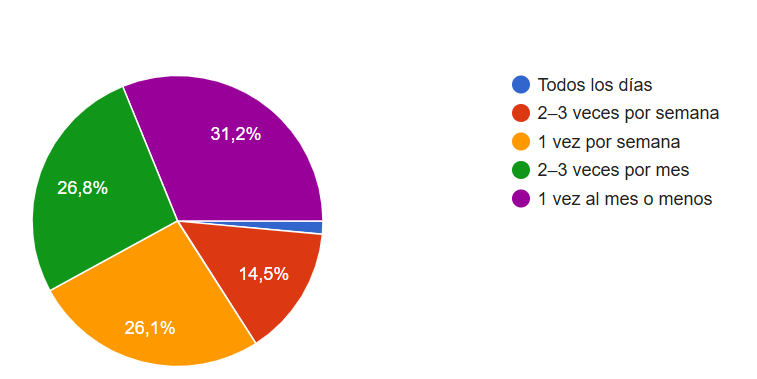
\includegraphics[width=0.78\textwidth]{images/FrecuenciaCompraPanificados.png}
    \caption{Frecuencia de compra de panificados. -- Fuente: elaboración propia}
    \label{fig:frecuencia-compra-panificados}
\end{figure}

La distribución horaria muestra una fuerte concentración durante la tarde. El 53,6\% de las compras se realizan entre 15–18 h, muy por encima de los demás horarios. Este patrón confirma un pico intradiario pronunciado que justifica que AIVA trate la hora como variable de alto peso en el pronóstico e integre interacciones con día de semana y clima; operativamente, habilita recomendaciones de reposición con la suficiente antelación antes del pico, alertas de quiebre y sugerencias de sustitución cuando el stock proyectado sea insuficiente, acciones que atacan el momento de mayor riesgo de ventas perdidas.

\begin{figure}[t]
    \centering
    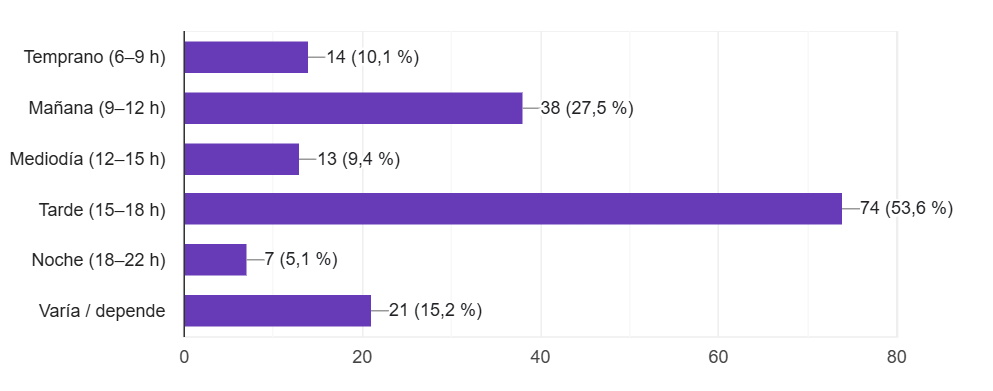
\includegraphics[width=0.78\textwidth]{images/MomentoDeCompra.png}
    \caption{Momento de compra de panificados. -- Fuente: elaboración propia}
    \label{fig:momento-compra}
\end{figure}


El 86,3\% de las personas declara comprar principalmente en panaderías/confiterías de barrio, lo que ubica al canal objetivo de AIVA exactamente donde se concentra la demanda. En ese mismo universo, al menos el 74,1\% experimentó algún faltante en el último mes. Esta combinación del canal dominante y alta incidencia de indisponibilidad, confirma la relevancia operativa del problema y respalda el diseño de AIVA: pronósticos por producto y franja horaria para panaderías de barrio, alertas tempranas de quiebre y sugerencias de sustitución para mitigar pérdidas justo donde más se compra.

\begin{figure}[t]
    \centering
    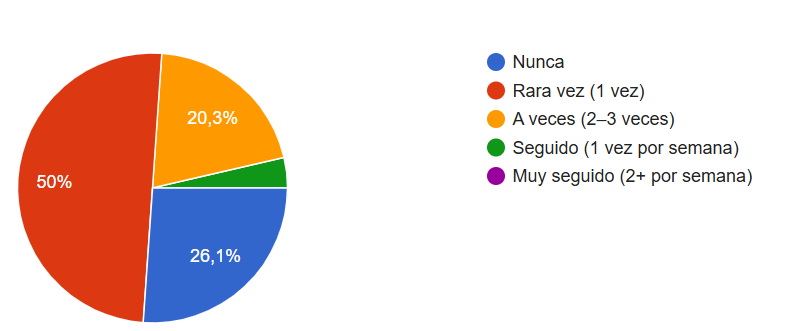
\includegraphics[width=0.78\textwidth]{images/NoHubieraProducto.png}
    \caption{Situación en la que faltó algún producto en la panadería. -- Fuente: elaboración propia}
    \label{fig:no-hubiera-producto}
\end{figure}


Ante la última situación de indisponibilidad, la mayoría reorientó la compra dentro del mismo local: 41,7\% eligió otra variedad/sabor y 28,1\% otro producto. En cambio, 25,9\% constituyó venta perdida. El 14,4\% se fue a otro local y 11,5\% no compró. Este patrón cuantifica tanto la oportunidad de retención como el costo del stockout. Para AIVA, estos datos respaldan un motor de sustituciones en tiempo real (sugerencias por afinidad y disponibilidad), alertas de quiebre y priorización de horneadas de los SKU críticos; además, permiten estimar pérdidas y monitorear la tasa de ventas perdidas como indicador operativo clave.


\begin{figure}[t]
    \centering
    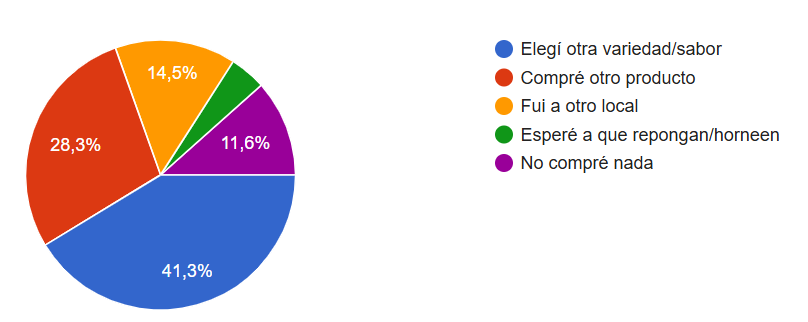
\includegraphics[width=0.78\textwidth]{images/AccionPosterior.png}
    \caption{Acción tomada por la persona al no conseguir el producto deseado. -- Fuente: elaboración propia}
    \label{fig:accion-posterior}
\end{figure}


El clima aparece como un factor determinante de la demanda: más de la mitad de las personas declara comprar más en días fríos (58\%) y lluviosos (55\%), mientras que en días calurosos predomina la disminución de compra (46\% “compro menos”). Este patrón confirma que las condiciones meteorológicas inciden de forma directa en el volumen a producir y cuándo hacerlo. En consecuencia, AIVA debe ponderar el clima como predictor de alto peso e integrar pronóstico de temperatura y precipitaciones para reforzar horneadas/reposiciones antes de los picos en frío/lluvia, y moderar lotes (con alertas y sustituciones) en calor, minimizando faltantes y sobreproducción.

\begin{figure}[t]
    \centering
    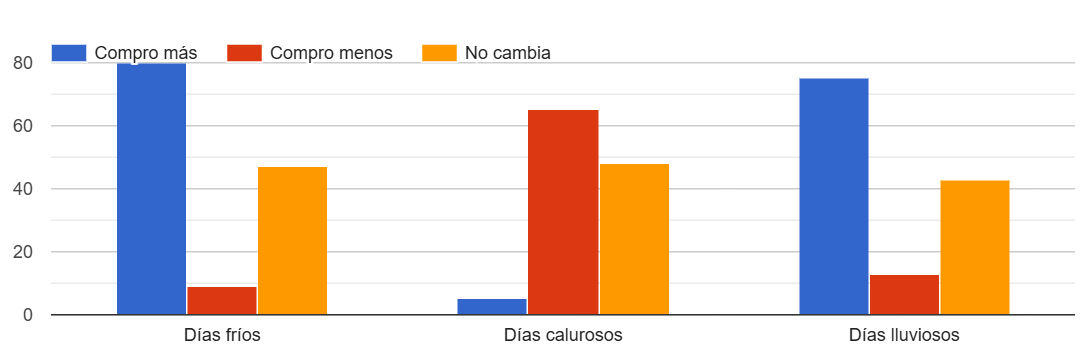
\includegraphics[width=0.78\textwidth]{images/CompraSegunClima.png}
    \caption{Frecuencia de compras según las condiciones climáticas. -- Fuente: elaboración propia}
    \label{fig:compras-segun-clima}
\end{figure}


La evidencia recolectada confirma que el problema de disponibilidad en panificados es real y frecuente. Tres de cada cuatro personas experimentaron algún faltante el último mes y, ante esa situación, alrededor de 1 de cada 4 casos termina en venta perdida. Estos resultados muestran que AIVA ataca un problema real, en el canal correcto y con funcionalidades que, según los datos, reducirán faltantes y mermas sin sobreproducir.


\subsection{Entrevista a Milena, encargada de la confitería ``La Catalana''}

Con el propósito de profundizar en el funcionamiento operativo de negocios dedicados a la elaboración y venta de productos perecederos, se realizó una entrevista a Milena González, encargada de la confitería \textit{La Catalana}, un establecimiento familiar con más de quince años de trayectoria en el rubro de la pastelería artesanal. El objetivo principal de la entrevista fue identificar las prácticas actuales de gestión de producción y demanda, así como los desafíos asociados al control de inventario y desperdicio de productos, con el fin de validar la pertinencia de una herramienta predictiva orientada a este tipo de comercios.

La Catalana cuenta con un equipo de 19 empleados y se especializa en la elaboración de una amplia variedad de productos de panadería y pastelería. Entre los más vendidos se destacan las tortas, los sandwichitos de miga y las facturas, mientras que los bombones y algunas masas finas registran una rotación menor. En promedio, los productos tienen una vida útil de entre dos y tres días: el pan se produce diariamente, y las porciones y masas se conservan durante un máximo de tres días, garantizando frescura pero también imponiendo la necesidad de una planificación precisa.

Actualmente, el negocio no utiliza ningún sistema formal de gestión o predicción. La estimación diaria de producción se realiza de forma empírica, basándose en la experiencia y el conocimiento del comportamiento de los clientes. Milena explicó que las decisiones se toman “intuitivamente”, considerando variables generales como el día de la semana o la proximidad de fines de semana, momentos en los cuales la demanda suele incrementarse.

En cuanto al registro histórico de ventas, La Catalana no cuenta con herramientas que permitan analizar los datos de manera sistemática. Esto representa una limitación relevante, ya que la ausencia de información consolidada impide realizar ajustes estratégicos en la producción y dificulta la detección de patrones de consumo. Milena remarcó la importancia de poder estimar con precisión la demanda, dado que los errores de cálculo generan pérdidas económicas al no poder comercializar a tiempo los productos elaborados.

Milena expresó además un claro interés en incorporar tecnologías que ayuden a optimizar la producción y reducir el desperdicio. Si bien actualmente no disponen de ninguna herramienta predictiva, considera que contar con un sistema que permita proyectar la demanda sería de gran ayuda para mejorar la eficiencia del negocio, evitar pérdidas y garantizar la disponibilidad de productos ante picos de demanda. Sin embargo, enfatizó que cualquier solución tecnológica debería ser “fácil e intuitiva de usar”, ya que el equipo no cuenta con una formación técnica avanzada.

En síntesis, la entrevista a Milena pone de manifiesto la necesidad de herramientas accesibles que faciliten la gestión de la producción en panaderías y confiterías tradicionales. Su testimonio refuerza la relevancia de desarrollar soluciones tecnológicas simples, pero efectivas, que permitan transformar la experiencia empírica de los dueños y encargados en decisiones basadas en datos. Esto valida el enfoque del presente proyecto, orientado a ofrecer una solución de predicción de demanda que contribuya a la eficiencia operativa y sostenibilidad económica de este tipo de negocios.


\subsection{Conclusión del user research}

La combinación de los resultados obtenidos a partir de la encuesta a consumidores y la entrevista en profundidad a una comerciante del rubro permitió validar empíricamente la necesidad y el potencial de una herramienta como AIVA.  

\indent Por un lado, la encuesta evidenció un patrón de consumo regular y predecible en el mercado de panificados, con picos de compra concentrados en franjas horarias específicas y una fuerte dependencia de variables externas como el clima y el día de la semana. Asimismo, se constató una alta frecuencia de faltantes: tres de cada cuatro personas experimentaron la ausencia de algún producto en el último mes, y en una de cada cuatro ocasiones esto derivó en una venta perdida. Este hallazgo cuantifica con claridad la magnitud del problema operativo que AIVA busca resolver: la ineficiencia en la planificación y reposición de productos perecederos.  

\indent Por otro lado, la entrevista con Milena González, encargada de la confitería \textit{La Catalana}, permitió comprender en profundidad las limitaciones cotidianas que enfrentan los comercios del sector. La ausencia de sistemas formales de registro y predicción obliga a basar la producción en la intuición y experiencia del personal, lo que incrementa el riesgo de sobreproducción o quiebre de stock. Sin embargo, la disposición expresada por Milena a incorporar soluciones tecnológicas simples y accesibles refuerza la viabilidad de adopción de AIVA dentro de este tipo de entornos.  

\indent En conjunto, ambos instrumentos de investigación —encuesta y entrevista— confirman que el problema de disponibilidad y desperdicio en panaderías y confiterías es real, frecuente y económicamente relevante. Además, validan la hipótesis central del proyecto: existe una oportunidad concreta para aplicar inteligencia artificial en la predicción de demanda de productos perecederos, generando beneficios medibles en eficiencia operativa, reducción de mermas y aumento de ventas.  

\indent Los hallazgos de esta etapa consolidan la base empírica sobre la cual se diseñará e implementará AIVA, asegurando que su arquitectura funcional y sus algoritmos respondan a las condiciones reales del mercado y a las necesidades específicas de los usuarios finales.

